\documentclass[
	usepdftitle=false,
	xcolor={table, dvipsnames},
	hyperref={
		pdftitle={Studio delle prestazioni di un Ufficio Postale ispirato a Poste Italiane},
    	pdfauthor={A. Chillotti, C. Cuffaro e S. Tiberi}
    }
]{beamer}

\mode<presentation> {

% The Beamer class comes with a number of default slide themes
% which change the colors and layouts of slides. Below this is a list
% of all the themes, uncomment each in turn to see what they look like.

%\usetheme{default}
%\usetheme{AnnArbor}
%\usetheme{Antibes}
%\usetheme{Bergen}
%\usetheme{Berkeley}
%\usetheme{Berlin}
%\usetheme{Boadilla}
%\usetheme{CambridgeUS}
%\usetheme{Copenhagen}
%\usetheme{Darmstadt}
%\usetheme{Dresden}
%\usetheme{Frankfurt}
%\usetheme{Goettingen}
%\usetheme{Hannover}
%\usetheme{Ilmenau}
%\usetheme{JuanLesPins}
%\usetheme{Luebeck}
\usetheme{Madrid}
%\usetheme{Malmoe}
%\usetheme{Marburg}
%\usetheme{Montpellier}
%\usetheme{PaloAlto}
%\usetheme{Pittsburgh}
%\usetheme{Rochester}
%\usetheme{Singapore}
%\usetheme{Szeged}
%\usetheme{Warsaw}

% As well as themes, the Beamer class has a number of color themes
% for any slide theme. Uncomment each of these in turn to see how it
% changes the colors of your current slide theme.

%\usecolortheme{albatross}
%\usecolortheme{beaver}
%\usecolortheme{beetle}
\usecolortheme{crane}
%\usecolortheme{dolphin}
%\usecolortheme{dove}
%\usecolortheme{fly}
%\usecolortheme{lily}
%\usecolortheme{orchid}
%\usecolortheme{rose}
%\usecolortheme{seagull}
%\usecolortheme{seahorse}
%\usecolortheme{whale}
%\usecolortheme{wolverine}

%\setbeamertemplate{footline} % To remove the footer line in all slides uncomment this line
%\setbeamertemplate{footline}[page number] % To replace the footer line in all slides with a simple slide count uncomment this line

%\setbeamertemplate{navigation symbols}{} % To remove the navigation symbols from the bottom of all slides uncomment this line
}

\usepackage[utf8]{inputenc}
\usepackage[italian]{babel}
\usepackage[T1]{fontenc}
\usepackage{graphicx}
\usepackage{booktabs}
\usepackage{subcaption}
\usepackage{accents}

\setlength{\arrayrulewidth}{0.1em}
\renewcommand{\arraystretch}{1.2}

\title[Progetto PMCSN]{Studio delle prestazioni di un ufficio postale ispirato a\\ \textbf{Poste Italiane}} 

\author{A. Chillotti
\and 
C. Cuffaro
\and 
S. Tiberi
}

\institute[]{Università degli studi di Roma Tor Vergata}
\date{15 Settembre 2021}

\newcommand{\uo}{\textsl{Unica Operazione}}
\newcommand{\pp}{\textsl{Pagamenti \& Prelievi}}
\newcommand{\sr}{\textsl{Spedizioni \& Ritiri}}
\newcommand{\ded}{{\color{red}\hat{k}}}

\usefonttheme[onlymath]{serif}
\graphicspath{ {./figs/} }
\definecolor{code_purple}{rgb}{0.5,0,0.35}

\begin{document}

\begin{frame}
\titlepage
\end{frame}

\begin{frame}
\frametitle{Indice}
\tableofcontents
\end{frame}

\section{Presentazione del caso di studi} 
\begin{frame}
\frametitle{Presentazione del caso di studi (1)}
\begin{block}{Tipologie di servizi erogati}
\begin{enumerate}
\item \uo{} (e.g. ricarica \textsl{PostePay}, invio raccomandata e pagamento di massimo tre bollettini)
\item \pp{} (e.g. pagamento di un numero arbitrario di bollettini, bollo auto e libretti)  
\item \sr{} (e.g. invio corrispondenza, lettere, pacchi e raccomandate)
\end{enumerate}
\end{block}

\begin{block}{Giornata lavorativa}
\begin{enumerate}
\item 8 ore di erogazione dei ticket
\item Periodo necessario a smaltire le richieste rimaste pendenti
\end{enumerate}
\end{block}
\end{frame}

\begin{frame}
\frametitle{Presentazione del caso di studi (2)}
\begin{block}{Regole di servizio}
\begin{enumerate}
\item I ticket di tipo \sr{} vengono serviti da uno sportello dedicato il quale, in assenza di questa tipologia, opera come gli altri
\item Ai ticket di tipo \uo{} viene assegnata una priorità maggiore di quelli \pp{}
\item I clienti titolari di un conto \textsl{BancoPosta} sono prioritari
\end{enumerate}
\end{block}

\begin{figure}[ht]
\centering
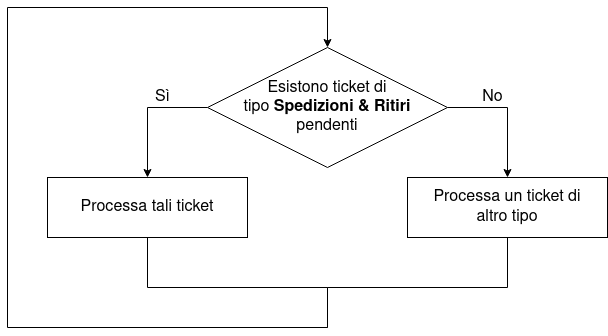
\includegraphics[width=0.5\linewidth]{presentazione-1}
\end{figure}
\end{frame}

\section{Obiettivi dello studio}
\begin{frame}
\frametitle{Obiettivi dello studio}
Minimizzare il numero $M$ degli sportelli operativi in un'intera giornata lavorativa, per garantire i seguenti QoS:

\begin{block}{Clienti titolari di un conto \textsl{BancoPosta}}
\begin{enumerate}
\item \uo{} $\to$ tempo medio d'attesa $\leq 5\ min$
\item \pp{} $\to$ tempo medio d'attesa $\leq 7.5\ min$
\item \sr{} $\to$ tempo medio d'attesa $\leq 10\ min$
\end{enumerate}
\end{block}

\begin{block}{Clienti \textbf{non} titolari di un conto \textsl{BancoPosta}}
\begin{enumerate}
\item \uo{} $\to$ tempo medio d'attesa $\leq 10\ min$
\item \pp{} $\to$ tempo medio d'attesa $\leq 12.5\ min$
\item \sr{} $\to$ tempo medio d'attesa $\leq 15\ min$
\end{enumerate}
\end{block}
\end{frame}

\section{Modello concettuale}
\begin{frame}
\frametitle{Modello concettuale (1)}
\begin{figure}[ht]
\centering
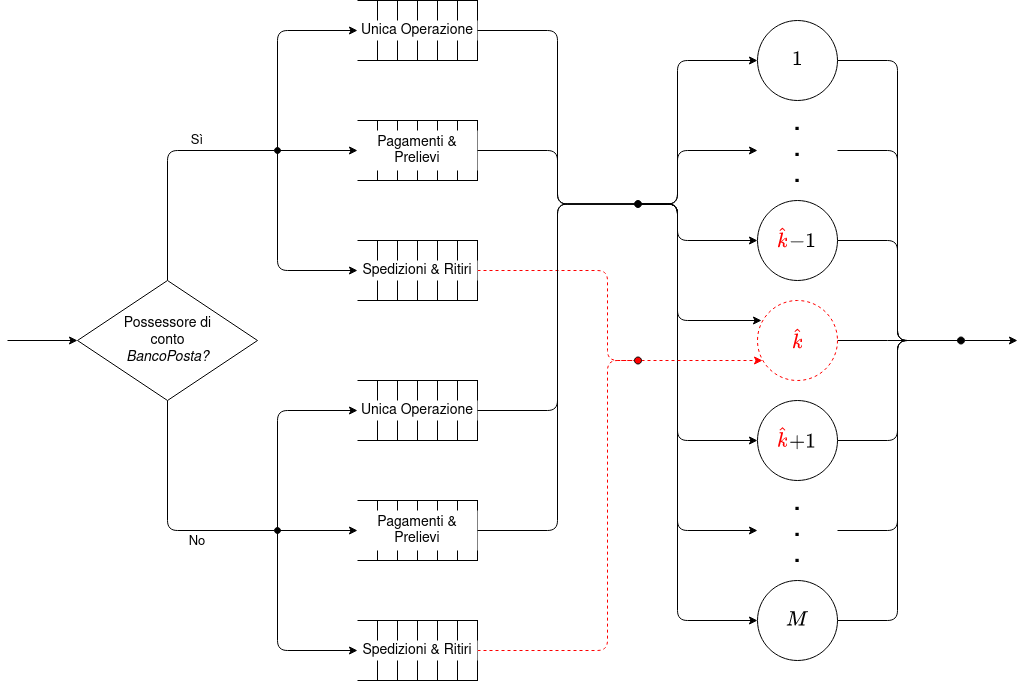
\includegraphics[width=0.8\linewidth]{modello-concettuale-1}
\end{figure}
\end{frame}

\begin{frame}
\frametitle{Modello concettuale (2)}
\begin{block}{Variabili di stato}
\begin{itemize}
\item Per ciascuno degli $M$ sportelli si ha:
\begin{equation*}
Server_r \in
\left\lbrace \mathtt{IDLE},\ \mathtt{BUSY} \right\rbrace
\end{equation*}
\item Per ciascuna delle 6 classi di utenza:
\begin{itemize}
\item Numero clienti totali della $c$-esima $\to$ $Customers_{c}$
\item Numero clienti in servizio della $c$-esima $\to$ $InService_{c}$
\end{itemize}
\end{itemize}
\end{block}

\begin{block}{Assunzioni}
\begin{itemize}
\item Comportamento di tipo \textsl{one-step}
\item Sistema \textsl{work conserving} (entro i vincoli imposti dal caso di studio)
\item Stato iniziale e finale:
\begin{equation*}
\begin{array}{c c c}
Server_r =\mathtt{IDLE}, & Customers_{c} = \mathtt{NONE}, & InService_{c} = \mathtt{NONE}
\end{array}
\end{equation*}
\end{itemize}
\end{block}
\end{frame}

\section{Modello delle specifiche}
\begin{frame}
\frametitle{Modello delle specifiche (1)}
\begin{block}{Variabili matematiche}
\begin{itemize}
\item Per ciascuno degli $M$ sportelli $\to Server_r(t) \in \lbrace 0, 1 \rbrace$
\item Per ciascuna delle 6 classi di utenza:
\begin{itemize}
\item Numero totale di clienti $\to Customers_c(t) \in \mathbb{N}$
\end{itemize}  
\item Per \uo{} e \pp{}:
\begin{itemize}
\item Numero di clienti in servizio $\to InService_c(t) \in \lbrace 0, 1, \dots, M \rbrace$
\end{itemize} 
Per \sr{}:
\begin{itemize}
\item Numero di clienti in servizio $\to InService_c(t) \in \lbrace 0, 1 \rbrace$
\end{itemize}
\end{itemize}
\end{block}

\begin{block}{Assunzioni}
\begin{itemize}
\item Distribuzione poissoniana degli arrivi
\item Distribuzione esponenziale dei tempi di interarrivo e di servizio
\item Disciplina FIFO delle code
\item Servizio senza prelazione
\end{itemize}
\end{block}
\end{frame}

\begin{frame}
\frametitle{Modello delle specifiche (2)}
\begin{block}{Probabilità}
\begin{itemize}
\item Probabilità di essere titolare di un conto \textsl{BancoPosta} $\to p_{BP} = 0.25$
\item Probabilità di acquisizione dei ticket:
\begin{equation*}
\begin{array}{c c c}
p_{UO} = 0.5, & p_{PP} = 0.35, & p_{SR} = 0.15
\end{array}
\end{equation*} 
\end{itemize}
\end{block}

\begin{block}{Tempi medi di servizio e d'arrivo}
\begin{itemize}
\item Tempo medio di servizio per tipologia di ticket:
\begin{equation*}
\begin{array}{l c l}
\uo{} & \rightarrow & 7\ min \\
\pp{} & \rightarrow & 14\ min \\
\sr{} & \rightarrow & 10\ min
\end{array}
\end{equation*} 
\item Tasso medio d'arrivo $\lambda = 0.243912\ req/min$ 
\end{itemize}
\end{block}
\end{frame}

\section{Modello computazionale}
\begin{frame}
\frametitle{Modello computazionale (1)}
\begin{block}{Variabili di programma}
\begin{itemize}
\item Numero totale di clienti per ciascuna classe $c \to$ \texttt{customers[c]}
\item Numero di clienti in servizio per ciascuna classe $c \to$ \texttt{in\_service[c]}
\item Stato del servente generale $r$-esimo $\to$ \texttt{gen\_status[r]}
\item Stato del servente dedicato $\to$ \texttt{ded\_status}
\end{itemize}
\end{block}
\begin{block}{Tipologie di eventi}
\begin{itemize}
\item Arrivo di un cliente afferente alla classe $c$
\item Completamento del servizio di un cliente della classe $c$ da parte di un server generale $r$
\item Completamento del servizio di un cliente della classe $c$ da parte del server dedicato
\end{itemize} 
\end{block}
\end{frame}

\begin{frame}
\frametitle{Modello computazionale (2)}
Campionamento delle statistiche:
\begin{block}{Time-averaged}
\begin{itemize}
\item Popolazione media nel centro $\to\bar{l}_c=\frac{1}{t_{end}}\int_0^{t_{end}} l_c(t) dt$
\item Popolazione media nella coda $\to\bar{q}_c=\frac{1}{t_{end}}\int_0^{t_{end}} q_c(t) dt$
\item Popolazione media in servizio $\to\bar{y}_c=\frac{1}{t_{end}}\int_0^{t_{end}} y_c(t) dt$
\end{itemize}
\end{block}
\begin{block}{Job-averaged}
\begin{itemize}
\item Tempo medio di interarrivo $\to\bar{r}_c = \frac{1}{n_c} \sum_{i=1}^{n_c} r_{c,i} = \frac{a_{n_c}}{n_c}$
\item Tempo medio di risposta $\to\bar{w}_c = \frac{1}{n_c} \sum_{i=1}^{n_c} w_{c,i}$
\item Tempo medio d'attesa $\to\bar{d}_c = \frac{1}{n_c} \sum_{i=1}^{n_c} d_{c,i}$
\item Tempo medio di servizio $\to\bar{s}_c = \frac{1}{n_c} \sum_{i=1}^{n_c} s_{c,i}$
\end{itemize}
\end{block}
\end{frame}

\section{Verifica}
\begin{frame}
\frametitle{Verifica (1)}
Comportamento del servente dedicato:
\begin{figure}[ht]
\centering
\begin{subfigure}[b]{0.475\textwidth}
\centering
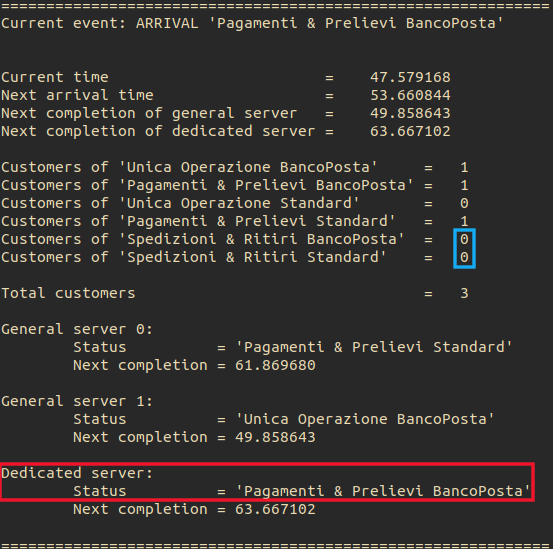
\includegraphics[width=\textwidth]{screenshots/original/ded_server_changes_behaviour}
\end{subfigure}
\hfill    
\begin{subfigure}[b]{0.475\textwidth}  
\centering 
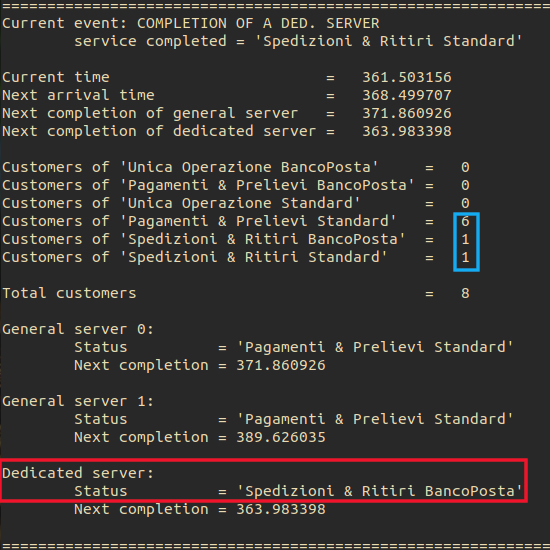
\includegraphics[width=\textwidth]{screenshots/original/ded_server_priority_sched}
\end{subfigure}
\end{figure}
\end{frame}

\begin{frame}
\frametitle{Verifica (2)}
Comportamento dei serventi generali:
\begin{figure}[ht]
\begin{subfigure}[b]{0.475\textwidth}   
\centering 
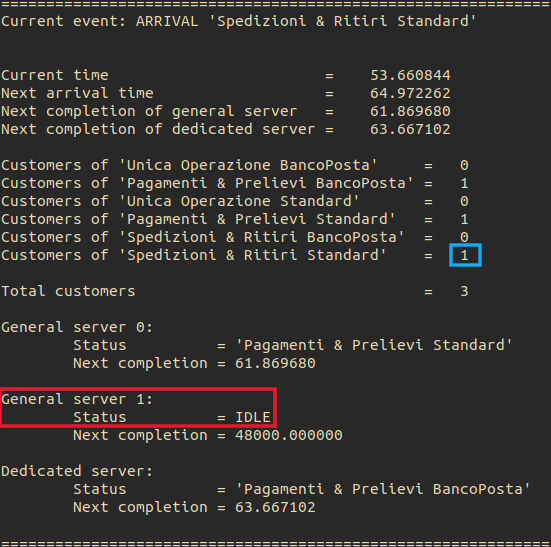
\includegraphics[width=\textwidth]{screenshots/original/gen_servers_no_SR}
\end{subfigure}
\hfill
\begin{subfigure}[b]{0.475\textwidth}   
\centering 
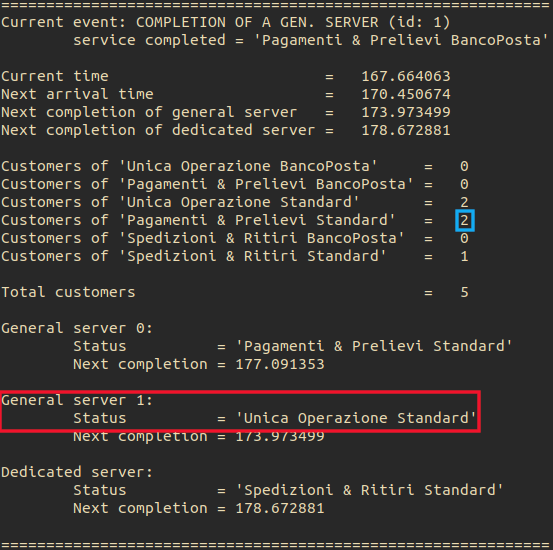
\includegraphics[width=\textwidth]{screenshots/original/gen_servers_priority_sched}
\end{subfigure}
\end{figure}
\end{frame}

\begin{frame}
\frametitle{Verifica (3)}
Controllo di consistenza sulle statistiche campionate:
\begin{figure}[ht]  
\centering 
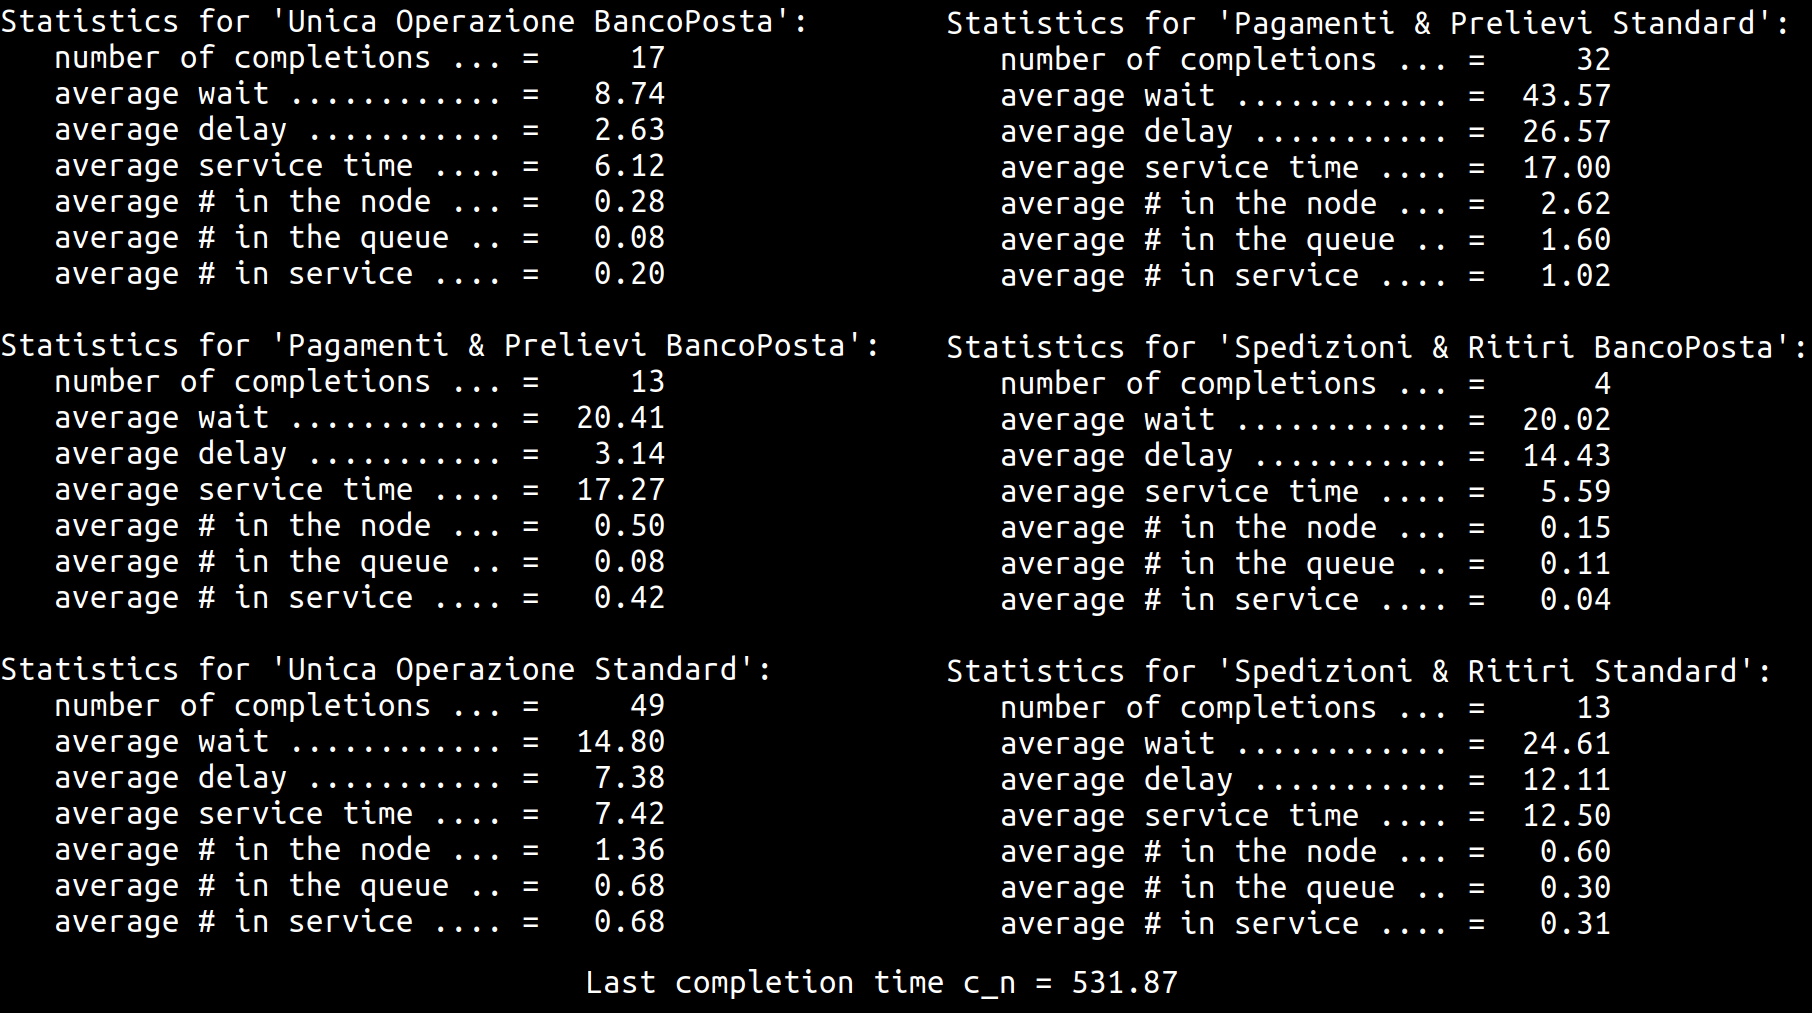
\includegraphics[width=\textwidth]{screenshots/original/statistics}
\end{figure}
\end{frame}

\section{Validazione}
\begin{frame}
\frametitle{Validazione (1)}
Blocco del flusso di tipo \sr{}
\vspace{2em}
\begin{columns}[c]
\column{0.45\textwidth}
\begin{figure}[ht]
\centering
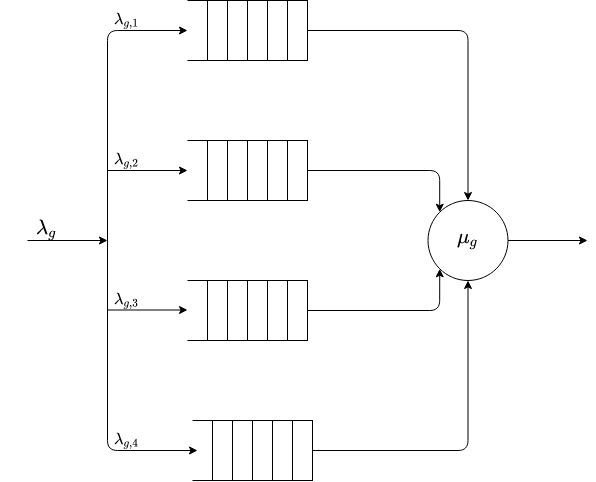
\includegraphics[width=\textwidth]{validazione-modello-analitico-1a}
\end{figure}
\column{0.45\textwidth}
Risultati analitici:
\begin{itemize}
\item $E[T_{Q_g}]^{KP} = 9.256825\ min$
\item $E[T_{S_g}] = 12.756807\ min$
\end{itemize}
Risultati della simulazione:
\begin{itemize}
\item $\bar{d}_g = (4.29 \pm 1.02)\ min$
\item $\bar{w}_g = (14.56 \pm 1.29)\ min$
\end{itemize}
\end{columns}
\end{frame}

\begin{frame}
\frametitle{Validazione (2)}
Blocco dei flussi di tipo \uo{} e \pp{}
\vspace{2em}
\begin{columns}[c]
\column{0.45\textwidth}
\begin{figure}[ht]
\centering
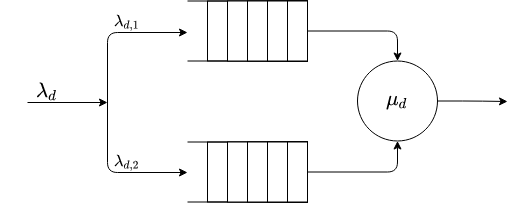
\includegraphics[width=\textwidth]{validazione-modello-analitico-1b}
\end{figure}
\column{0.45\textwidth}
Risultati analitici:
\begin{itemize}
\item $E[T_{Q_d}]^{KP} = 5.769637\ min$
\item $E[T_{S_d}] = 15.769637\ min$
\end{itemize}
Risultati della simulazione:
\begin{itemize}
\item $\bar{d}_d = (6.04 \pm 1.88)\ min$
\item $\bar{w}_d = (16.45 \pm 2.64)\ min$
\end{itemize}
\end{columns}
\end{frame}

\section{Esperimenti di simulazione}
\begin{frame}
\frametitle{Esperimenti di simulazione (1)}
\begin{block}{Numero minimo di sportelli}
\begin{itemize}
\item \textbf{Obiettivo}: trovare il minimo $M$ che soddisfi i QoS ($M^*$)
\item \textbf{Durata simulazione}: intera giornata lavorativa
\item \textbf{Tipologia di simulazione}: orizzonte finito
\item \textbf{Tecnica di simulazione}: replication
\item \textbf{Numero di repliche}: 10000
\item \textbf{Istante di campionamento}: al termine di ogni replica
\item \textbf{Seme iniziale}: 9
\item \textbf{Livello di confidenza degli intervalli}: 95 \%
\end{itemize}
\end{block}
\end{frame}

\begin{frame}
\frametitle{Esperimenti di simulazione (2)}
\begin{figure}[ht]
\centering
\begin{subfigure}[b]{0.3\textwidth}
\centering
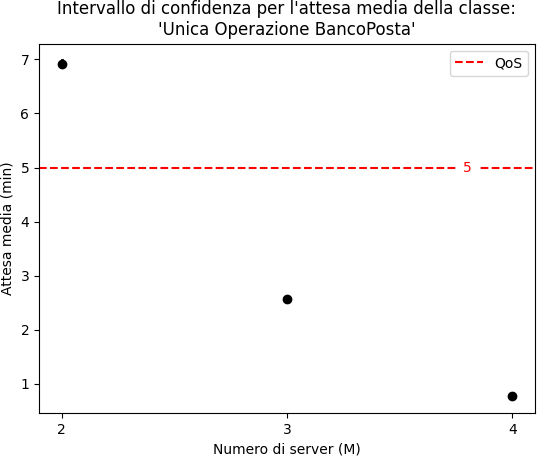
\includegraphics[width=\textwidth]{plots/d0-trans}
\end{subfigure}    
\begin{subfigure}[b]{0.3\textwidth}  
\centering 
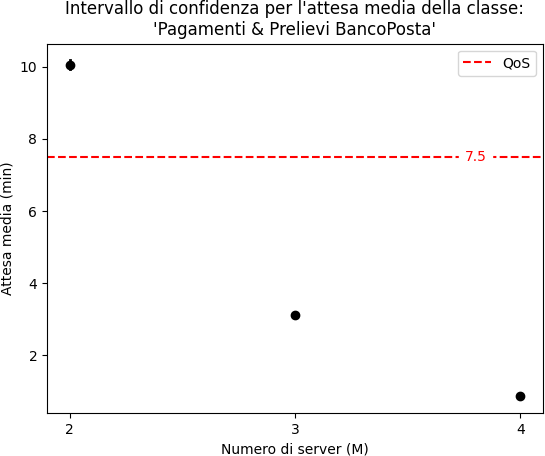
\includegraphics[width=\textwidth]{plots/d1-trans}   
\end{subfigure}
\begin{subfigure}[b]{0.3\textwidth}   
\centering 
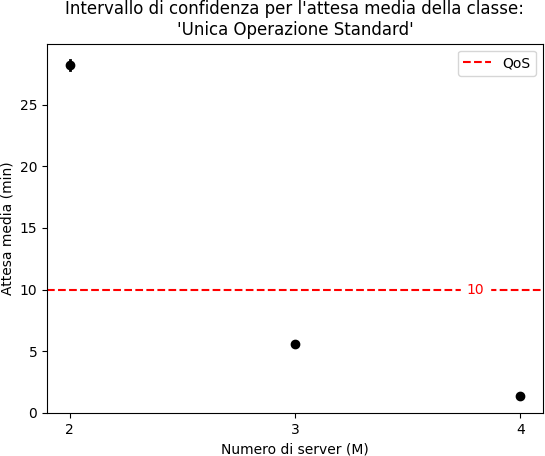
\includegraphics[width=\textwidth]{plots/d2-trans}
\end{subfigure}
\vskip\baselineskip
\begin{subfigure}[b]{0.3\textwidth}
\centering
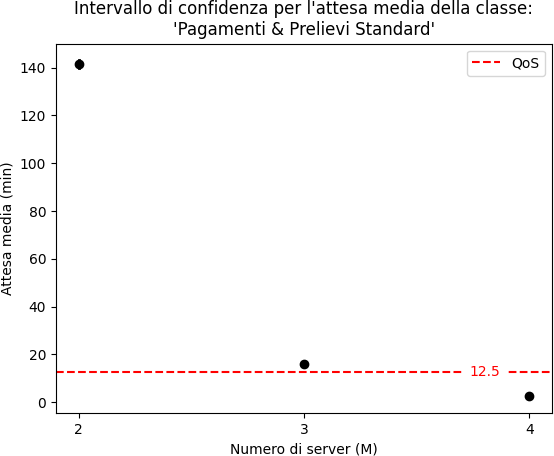
\includegraphics[width=\textwidth]{plots/d3-trans}
\end{subfigure}    
\begin{subfigure}[b]{0.3\textwidth}  
\centering 
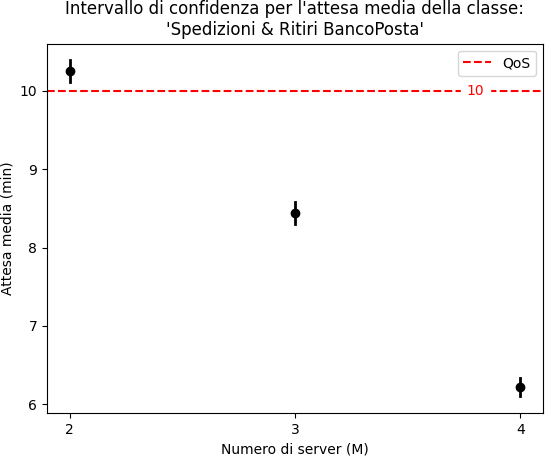
\includegraphics[width=\textwidth]{plots/d4-trans}   
\end{subfigure}
\begin{subfigure}[b]{0.3\textwidth}   
\centering 
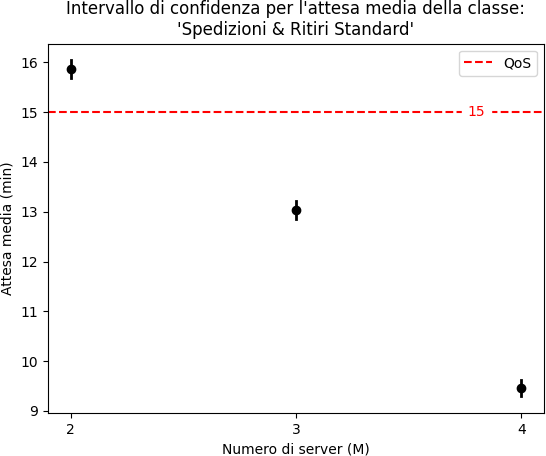
\includegraphics[width=\textwidth]{plots/d5-trans}
\end{subfigure}
\end{figure}
\end{frame}

\begin{frame}
\frametitle{Esperimenti di simulazione (3)}
\begin{block}{Andamento dell'attesa nell'arco della giornata}
\begin{itemize}
\item \textbf{Obiettivo}: studiare l'evoluzione dell'attesa media in funzione di $M^*$
\item \textbf{Durata simulazione}: intera giornata lavorativa
\item \textbf{Tipologia di simulazione}: orizzonte finito
\item \textbf{Tecnica di simulazione}: replication
\item \textbf{Numero di repliche}: 10000
\item \textbf{Istante di campionamento}: ogni ora per ciascuna replica
\item \textbf{Seme iniziale}: 9
\item \textbf{Livello di confidenza degli intervalli}: 95 \%
\end{itemize}
\end{block}
\end{frame}

\begin{frame}
\frametitle{Esperimenti di simulazione (4)}
\begin{figure}[ht]
\centering
\begin{subfigure}[b]{0.3\textwidth}
\centering
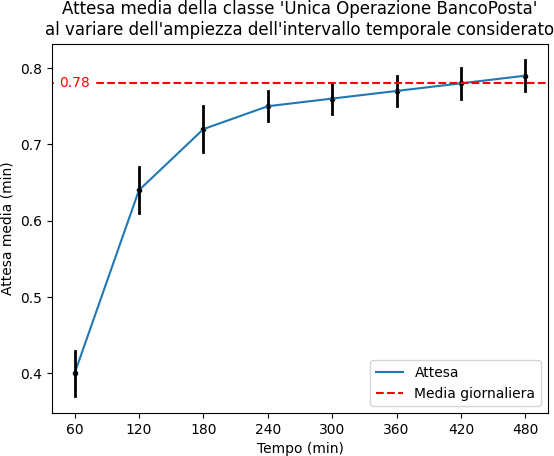
\includegraphics[width=\textwidth]{plots/day-from-empty-0}
\end{subfigure}
\begin{subfigure}[b]{0.3\textwidth}  
\centering 
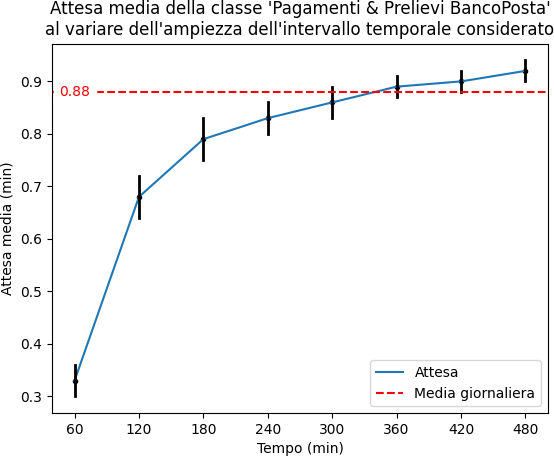
\includegraphics[width=\textwidth]{plots/day-from-empty-1}
\end{subfigure}
\begin{subfigure}[b]{0.3\textwidth}   
\centering 
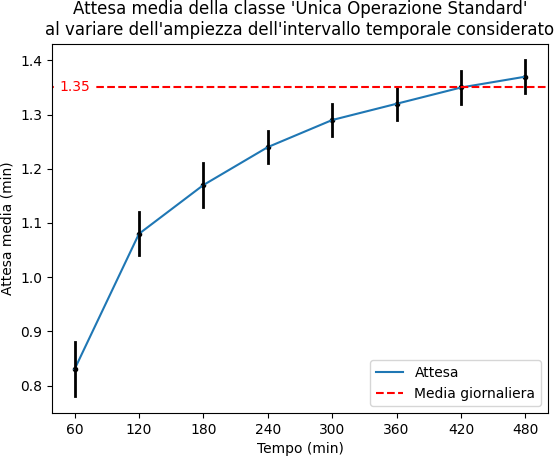
\includegraphics[width=\textwidth]{plots/day-from-empty-2}
\end{subfigure}
\vskip\baselineskip
\begin{subfigure}[b]{0.3\textwidth}   
\centering 
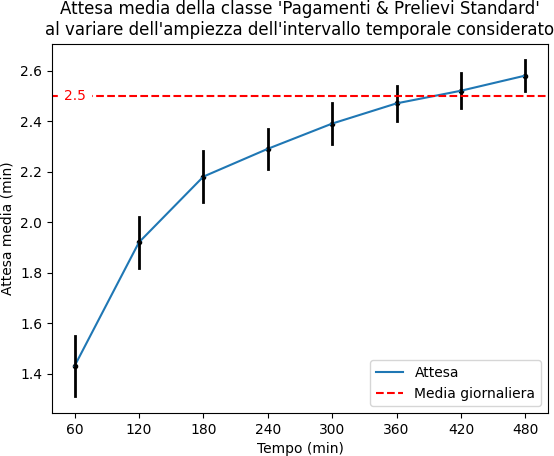
\includegraphics[width=\textwidth]{plots/day-from-empty-3}
\end{subfigure}
\begin{subfigure}[b]{0.3\textwidth}   
\centering 
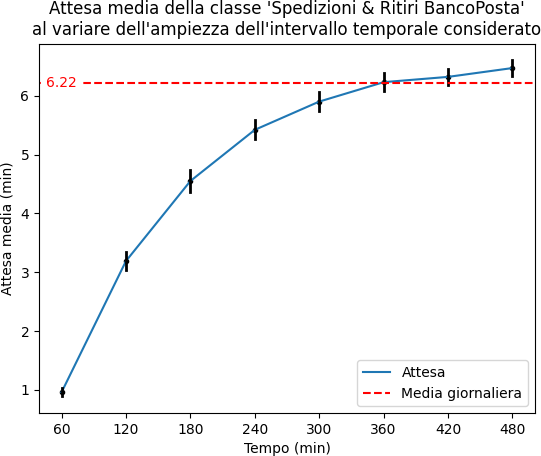
\includegraphics[width=\textwidth]{plots/day-from-empty-4}   
\end{subfigure}
\begin{subfigure}[b]{0.3\textwidth}   
\centering 
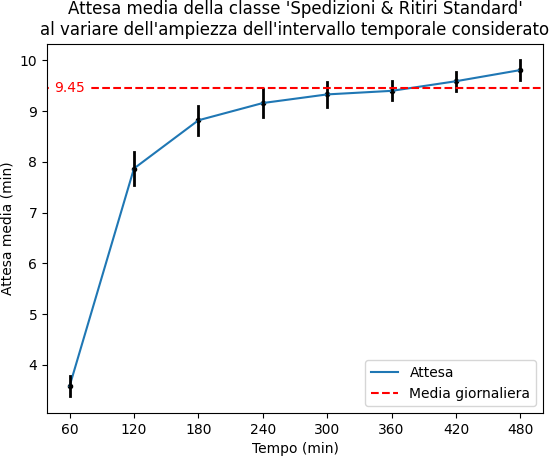
\includegraphics[width=\textwidth]{plots/day-from-empty-5}    
\end{subfigure}
\end{figure}
\end{frame}

\begin{frame}
\frametitle{Esperimenti di simulazione (5)}
\begin{figure}[ht]
\centering
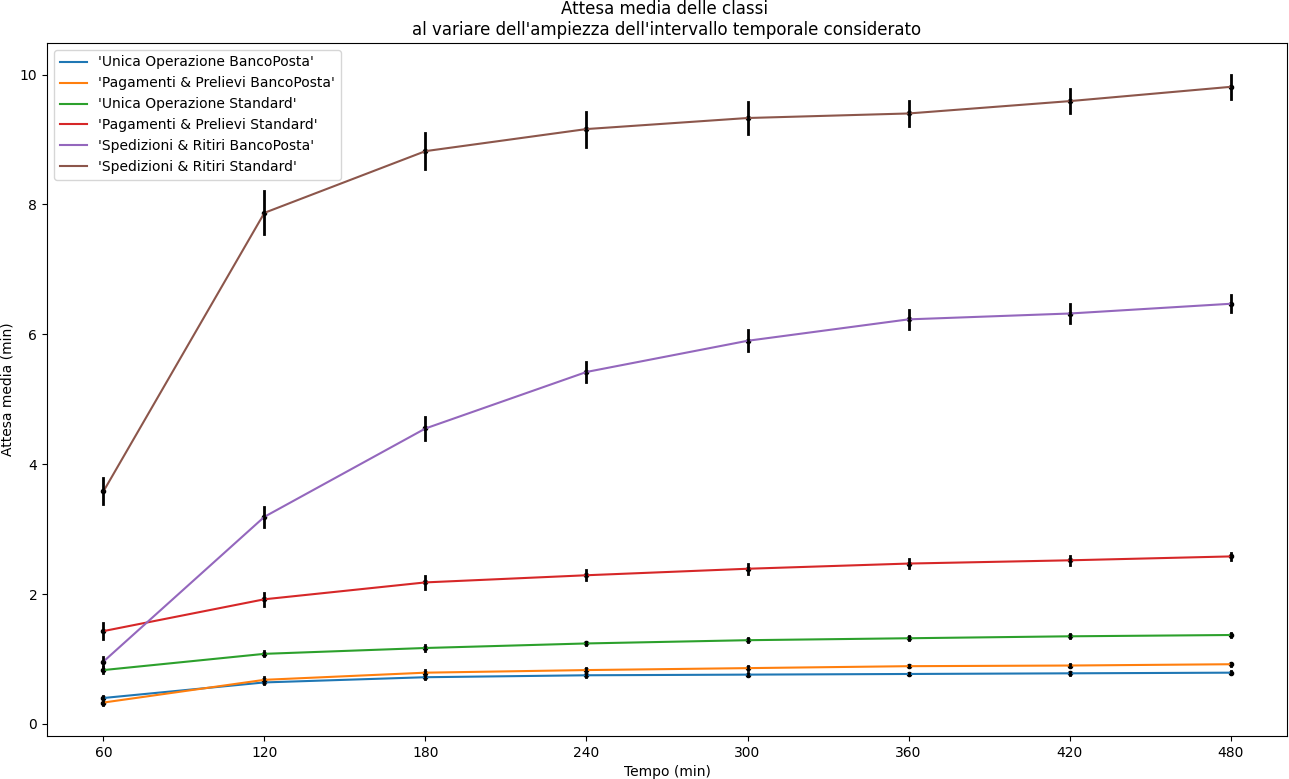
\includegraphics[width=\textwidth]{plots/day-from-empty-all}
\end{figure}
\end{frame}

\begin{frame}
\frametitle{Esperimenti di simulazione (6)}
\begin{block}{Mancato raggiungimento dello stato stazionario}
\begin{itemize}
\item \textbf{Obiettivo}: mostrare il mancato raggiungimento della stazionarietà all'interno della singola giornata lavorativa
\item \textbf{Durata simulazione}: due giornate lavorative
\item \textbf{Tipologia di simulazione}: orizzonte finito
\item \textbf{Tecnica di simulazione}: replication
\item \textbf{Numero di repliche}: 10000
\item \textbf{Istante di campionamento}: al termine di ogni replica
\item \textbf{Seme iniziale}: 9
\item \textbf{Livello di confidenza degli intervalli}: 95 \%
\end{itemize}
\end{block}
\end{frame}

\begin{frame}
\frametitle{Esperimenti di simulazione (7)}
\begin{figure}[ht]
\centering
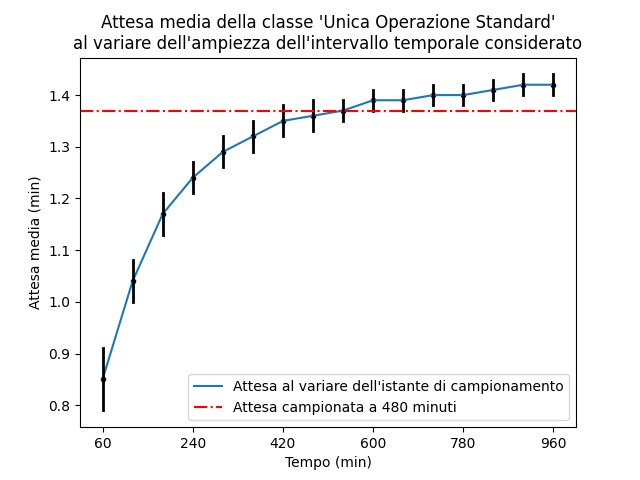
\includegraphics[width=0.7\textwidth]{plots/d2-no-stat}
\end{figure}
\end{frame}

\begin{frame}
\frametitle{Esperimenti di simulazione (8)}
\begin{block}{Analisi dei risultati}
\begin{itemize}
\item Il numero minimo di serventi necessari è $M^*=4$
\item Dopo circa 5 ore dall'apertura del centro postale, l'attesa media si avvicina al valore medio calcolato sull'intera giornata lavorativa per tutte le classi
\item I tempi d'attesa per le classi \sr{} \textsl{BancoPosta} e \textsl{Standard} sono di un ordine di grandezza superiore a quelli delle restanti, perché serviti dal singolo servente dedicato piuttosto che da un multiserver
\item Il tempo medio d'attesa per la classe \uo{} \textsl{Standard} continua a crescere dopo i primi $480$ minuti, per cui non viene raggiunta la stazionarietà nella singola giornata lavorativa
\end{itemize}
\end{block}
\end{frame}

\section{Miglioria}

\begin{frame}
\frametitle{Miglioria (1)}
\begin{block}{Definizioni preliminari}
\begin{itemize}
\item $A$ un cliente titolare di un conto \textsl{BancoPosta}, possessore di un ticket di tipo \uo{} o \pp{}
\item $B$ un cliente \textbf{non} titolare di un conto \textsl{BancoPosta}, possessore di un ticket di tipo \uo{} o \pp{}
\item $C$ un cliente possessore di un ticket di tipo \sr{}
\end{itemize}
\end{block}
\begin{block}{Regole aggiuntive}
\begin{itemize}
\item Dopo ogni cliente di tipo $A$ servito, gli sportelli non dedicati servono, se presente, uno di tipo $B$, privilegiando la fila più lunga 
\item Dopo ogni 4 clienti di tipo $C$ serviti, lo sportello dedicato serve, se presente, uno di tipo $B$, privilegiando la fila più lunga
\item Nel caso in cui non vi siano clienti di tipo $C$ da servire, lo sportello dedicato dà priorità a quelli di tipo $B$, privilegiando la fila più lunga
\end{itemize}
\end{block}
\end{frame}

\begin{frame}
\frametitle{Miglioria (2)}
\begin{block}{\textbf{Esperimento}: numero minimo di sportelli}
\begin{itemize}
\item \textbf{Obiettivo}: trovare il minimo $M$ che soddisfi i QoS ($\accentset{\sim}{M} < M^*$)
\item \textbf{Durata simulazione}: intera giornata lavorativa
\item \textbf{Tipologia di simulazione}: orizzonte finito
\item \textbf{Tecnica di simulazione}: replication
\item \textbf{Numero di repliche}: 10000
\item \textbf{Istante di campionamento}: al termine di ogni replica
\item \textbf{Seme iniziale}: 9
\item \textbf{Livello di confidenza degli intervalli}: 95 \%
\end{itemize}
\end{block}
\end{frame}

\begin{frame}
\frametitle{Miglioria (3)}
\begin{figure}[ht]
\centering
\begin{subfigure}[b]{0.3\textwidth}
\centering
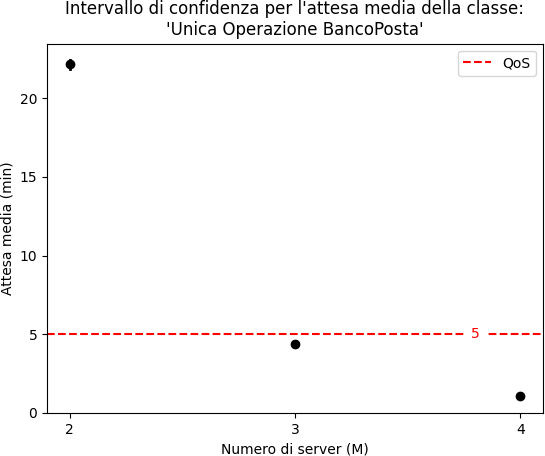
\includegraphics[width=\textwidth]{plots/d0-trans-imp}
\end{subfigure}    
\begin{subfigure}[b]{0.3\textwidth}  
\centering 
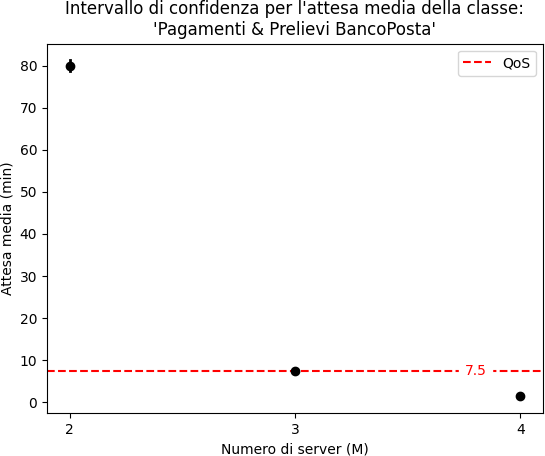
\includegraphics[width=\textwidth]{plots/d1-trans-imp}
\end{subfigure}
\begin{subfigure}[b]{0.3\textwidth}   
\centering 
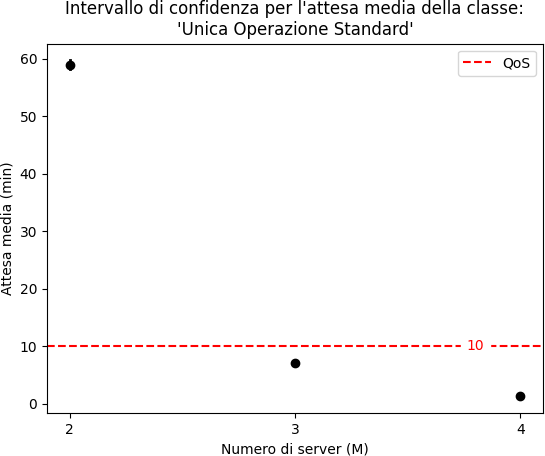
\includegraphics[width=\textwidth]{plots/d2-trans-imp}
\end{subfigure}
\vskip\baselineskip
\begin{subfigure}[b]{0.3\textwidth}   
\centering 
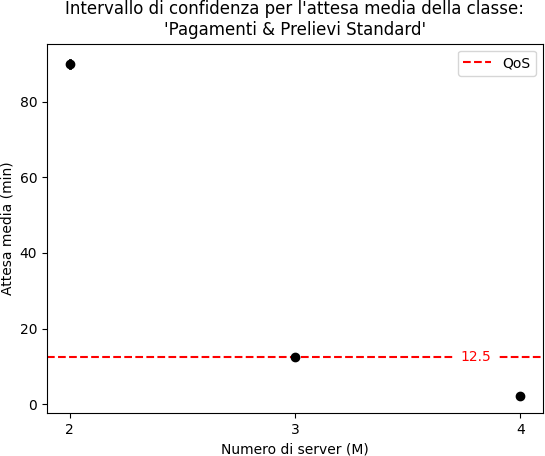
\includegraphics[width=\textwidth]{plots/d3-trans-imp}
\end{subfigure}
\begin{subfigure}[b]{0.3\textwidth}   
\centering 
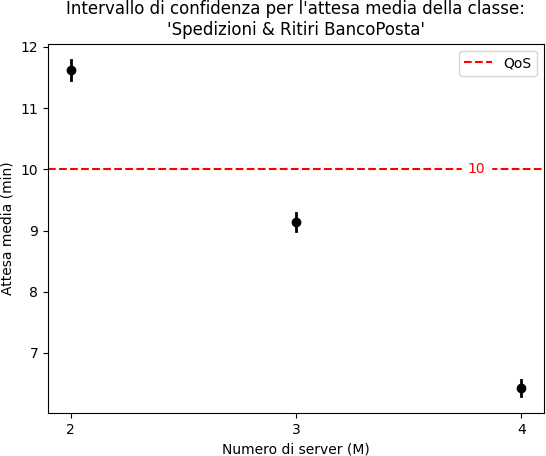
\includegraphics[width=\textwidth]{plots/d4-trans-imp}
\end{subfigure}
\begin{subfigure}[b]{0.3\textwidth}   
\centering 
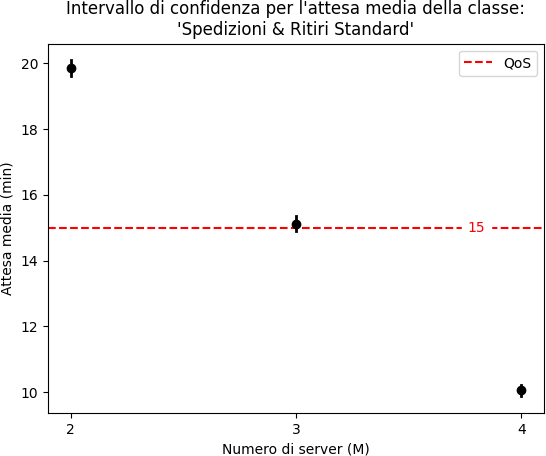
\includegraphics[width=\textwidth]{plots/d5-trans-imp}
\end{subfigure}
\end{figure}
\end{frame}

\begin{frame}
\frametitle{Miglioria (4)}
\begin{block}{Conclusioni}
Dallo studio effettuato è emerso come:
\begin{itemize}
\item Il sistema originale necessita di 4 sportelli operativi per soddisfare i QoS ($M^* = 4$)
\item La miglioria permette di diminuire di una unità il numero di sportelli operativi ($\accentset{\sim}M = 3$)
\end{itemize}
\vspace{1em}
Si suggerisce dunque l'adozione dell'algoritmo migliorativo, poiché:
\begin{itemize}
\item Consente di ridurre il numero minimo di sportelli da mantenere operativi
\item Permette di limitare l'investimento economico da parte del fornitore dei servizi
\end{itemize}
\end{block}
\end{frame}

\end{document} 